\chapter{Results}
\label{chap:Results}

\section{Observation}

As described in Sec.~\ref{sec:Optimization} above, the $L_\textrm{T} + \MET$ variable is a very efficient discriminator between the seesaw signal and the SM background. Therefore, the only requirement for the seesaw signal candidate events beyond the preliminary selection described in Sec.~\ref{sec:Selection} is that their $L_\textrm{T} + \MET$ value exceed 350\GeV. In Fig.~\ref{fig:Results} we present the $L_\textrm{T} + \MET$ distribution for four event categories as follows: 3 leptons with OSSF pair on-Z; 3 leptons with OSSF pair above-Z; 3 leptons with no OSSF pair; 4 leptons with at least one OSSF pair. Displays of the seesaw signal for heavy fermion mass $m_\Sigma = 420\GeV$ are also shown for each category. The signal generally stands out for higher values of $L_\textrm{T} + \MET$, as is to be expected for a massive parent particle. The SM background decomposition is also shown for each category.

\begin{sidewaysfigure}
\begin{center}
	\begin{subfigure}[b]{.5\textwidth}
		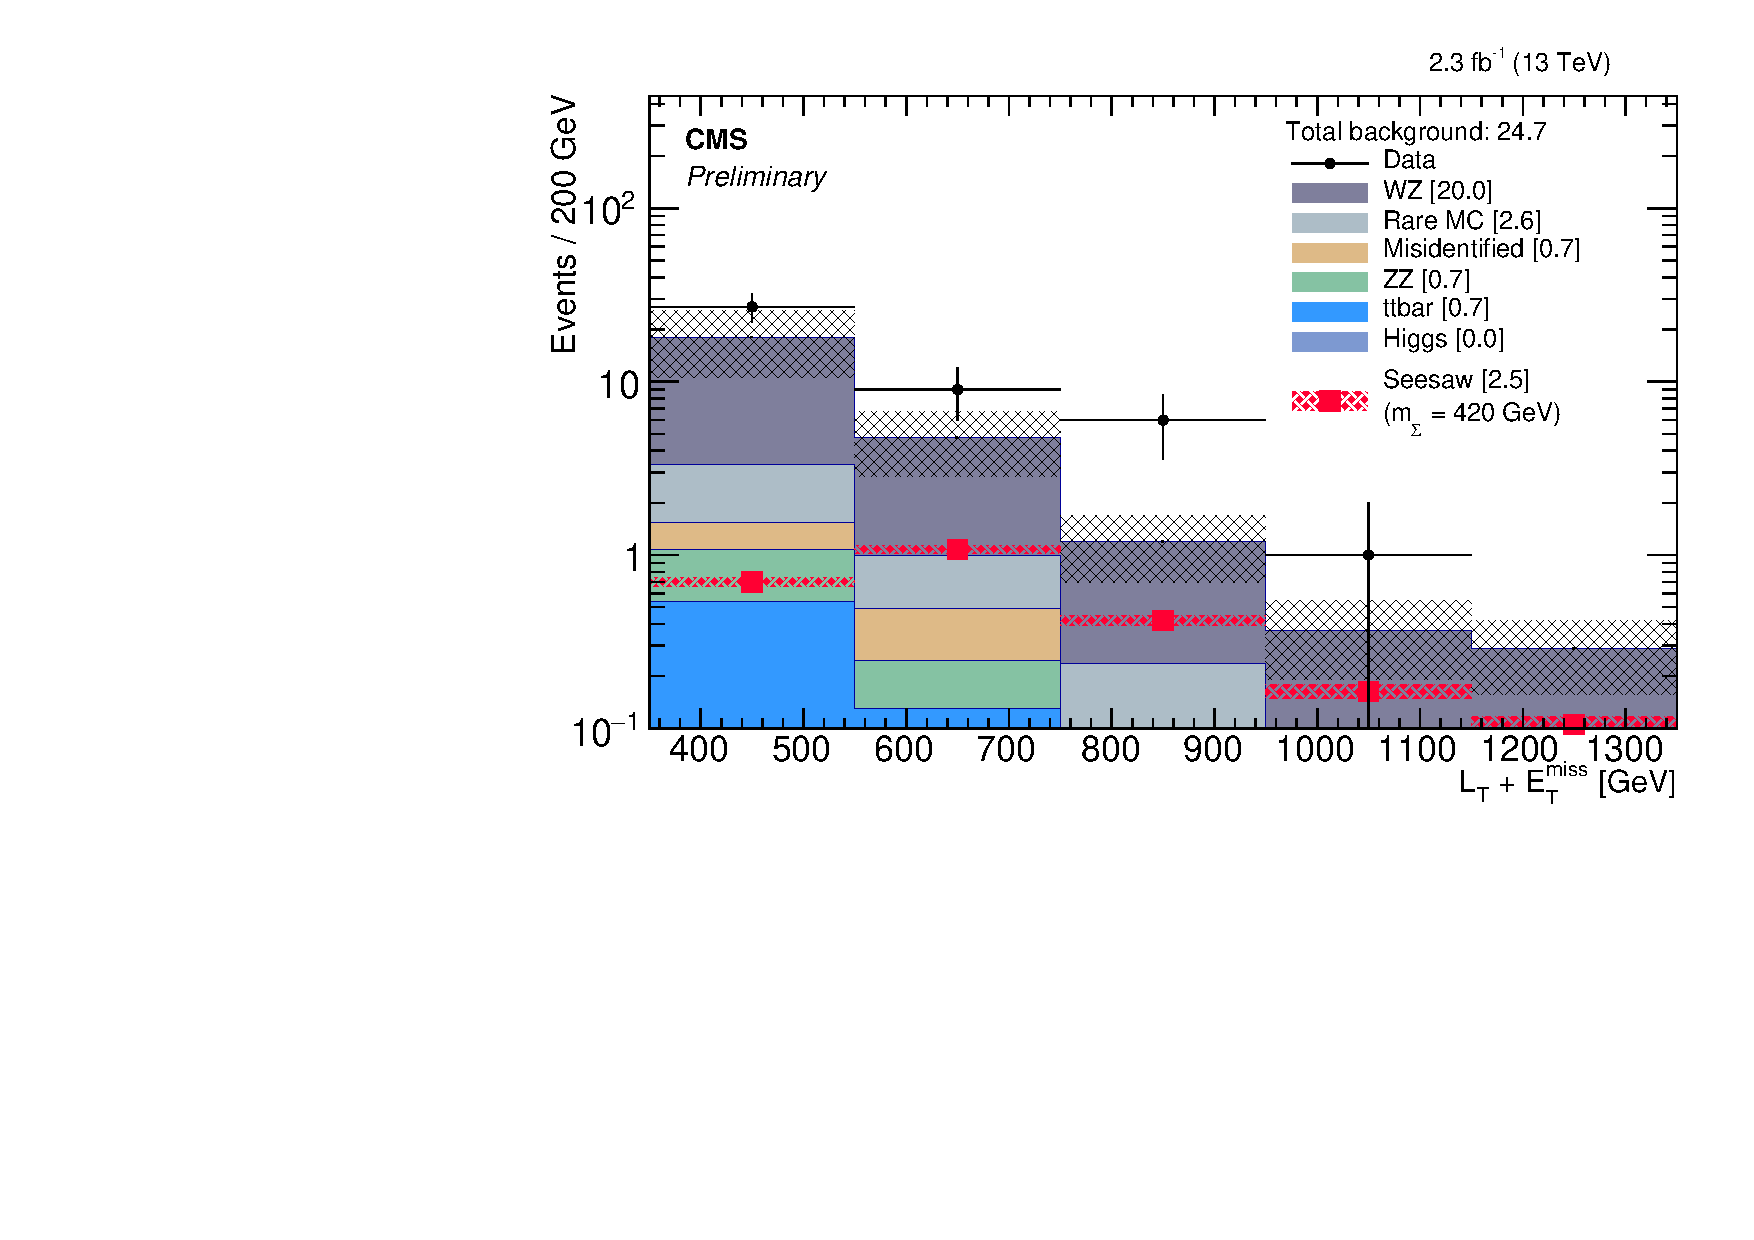
\includegraphics[width=\textwidth]{Results/plots/L3DYz1}
		\caption{3 leptons with OSSF pair on-\Z} \label{fig:Results/a}
	\end{subfigure}%
	\begin{subfigure}[b]{.5\textwidth}
		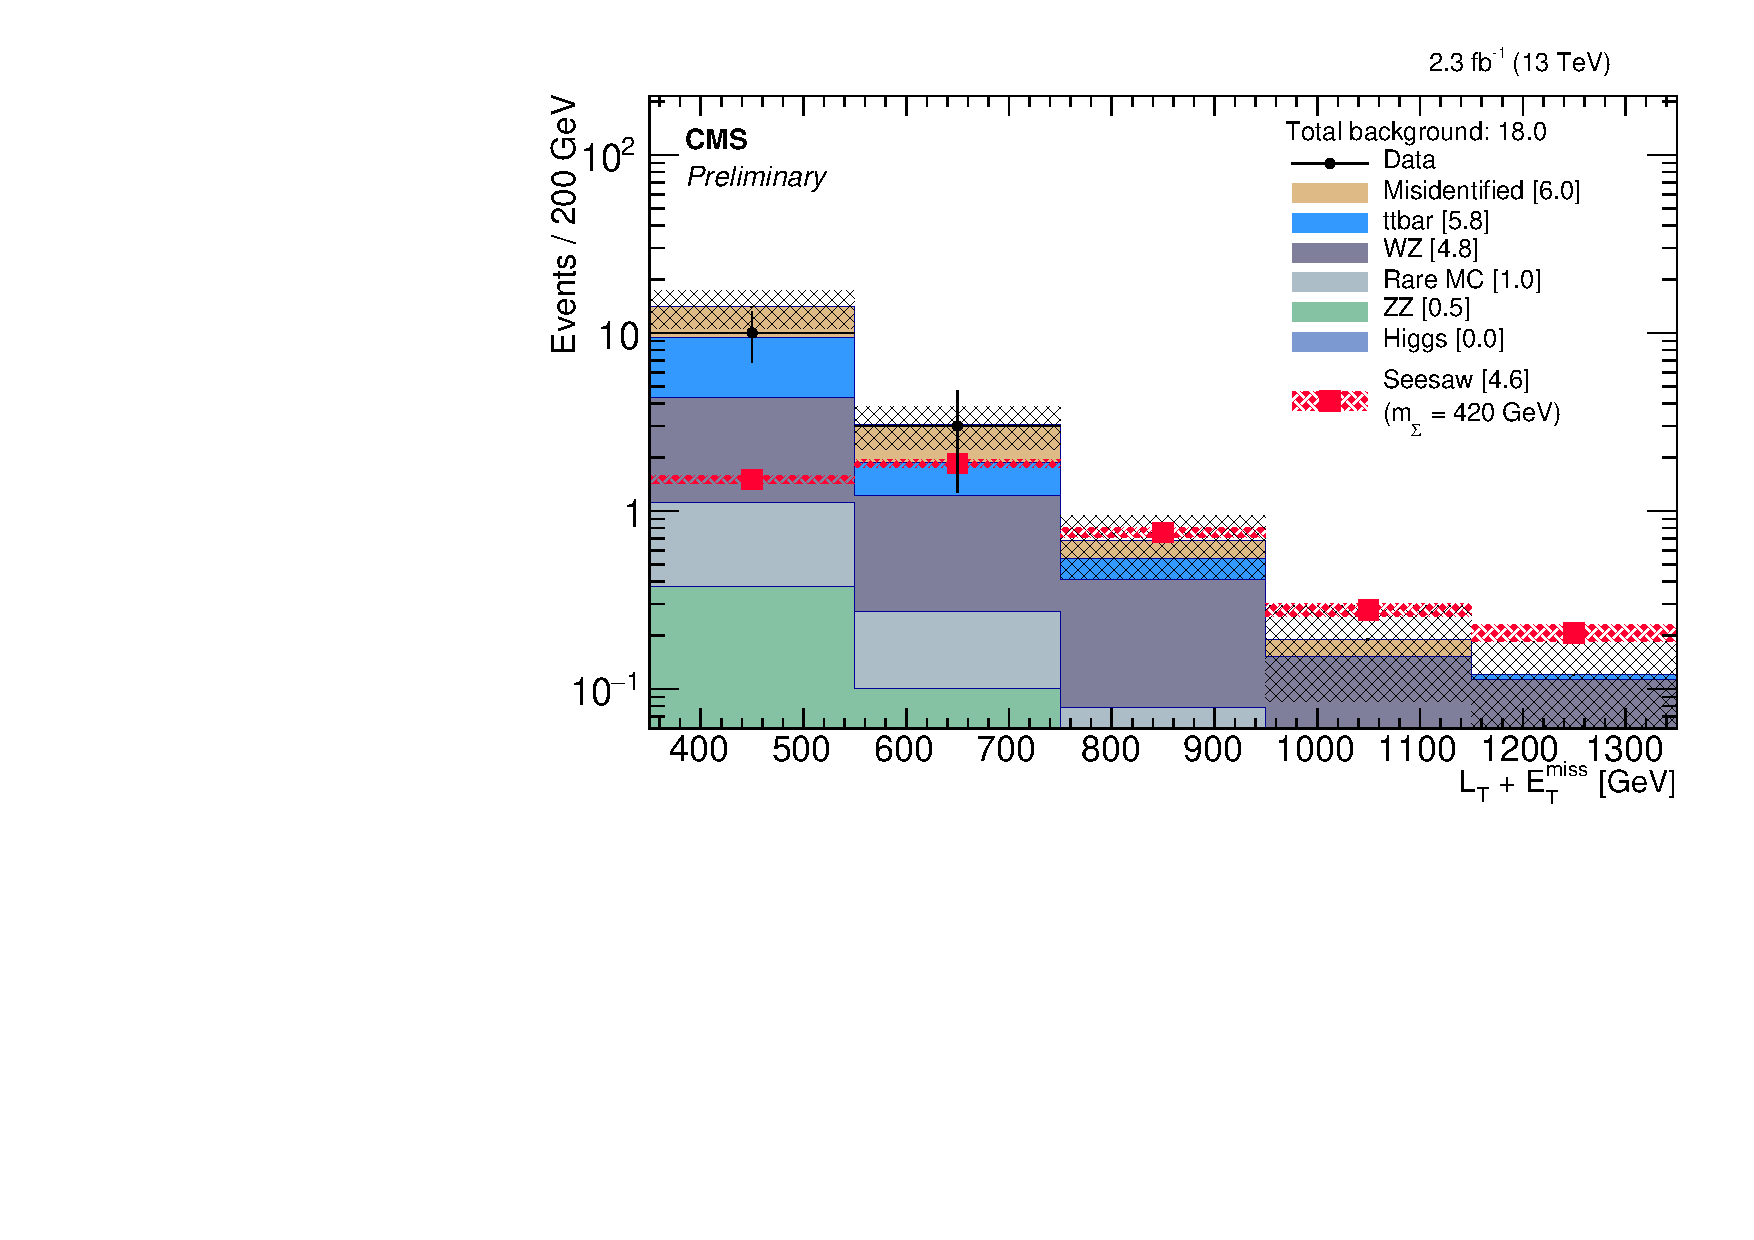
\includegraphics[width=\textwidth]{Results/plots/L3DYh1}
		\caption{3 leptons with OSSF pair above-\Z}
	\end{subfigure}
	\begin{subfigure}[b]{.5\textwidth}
		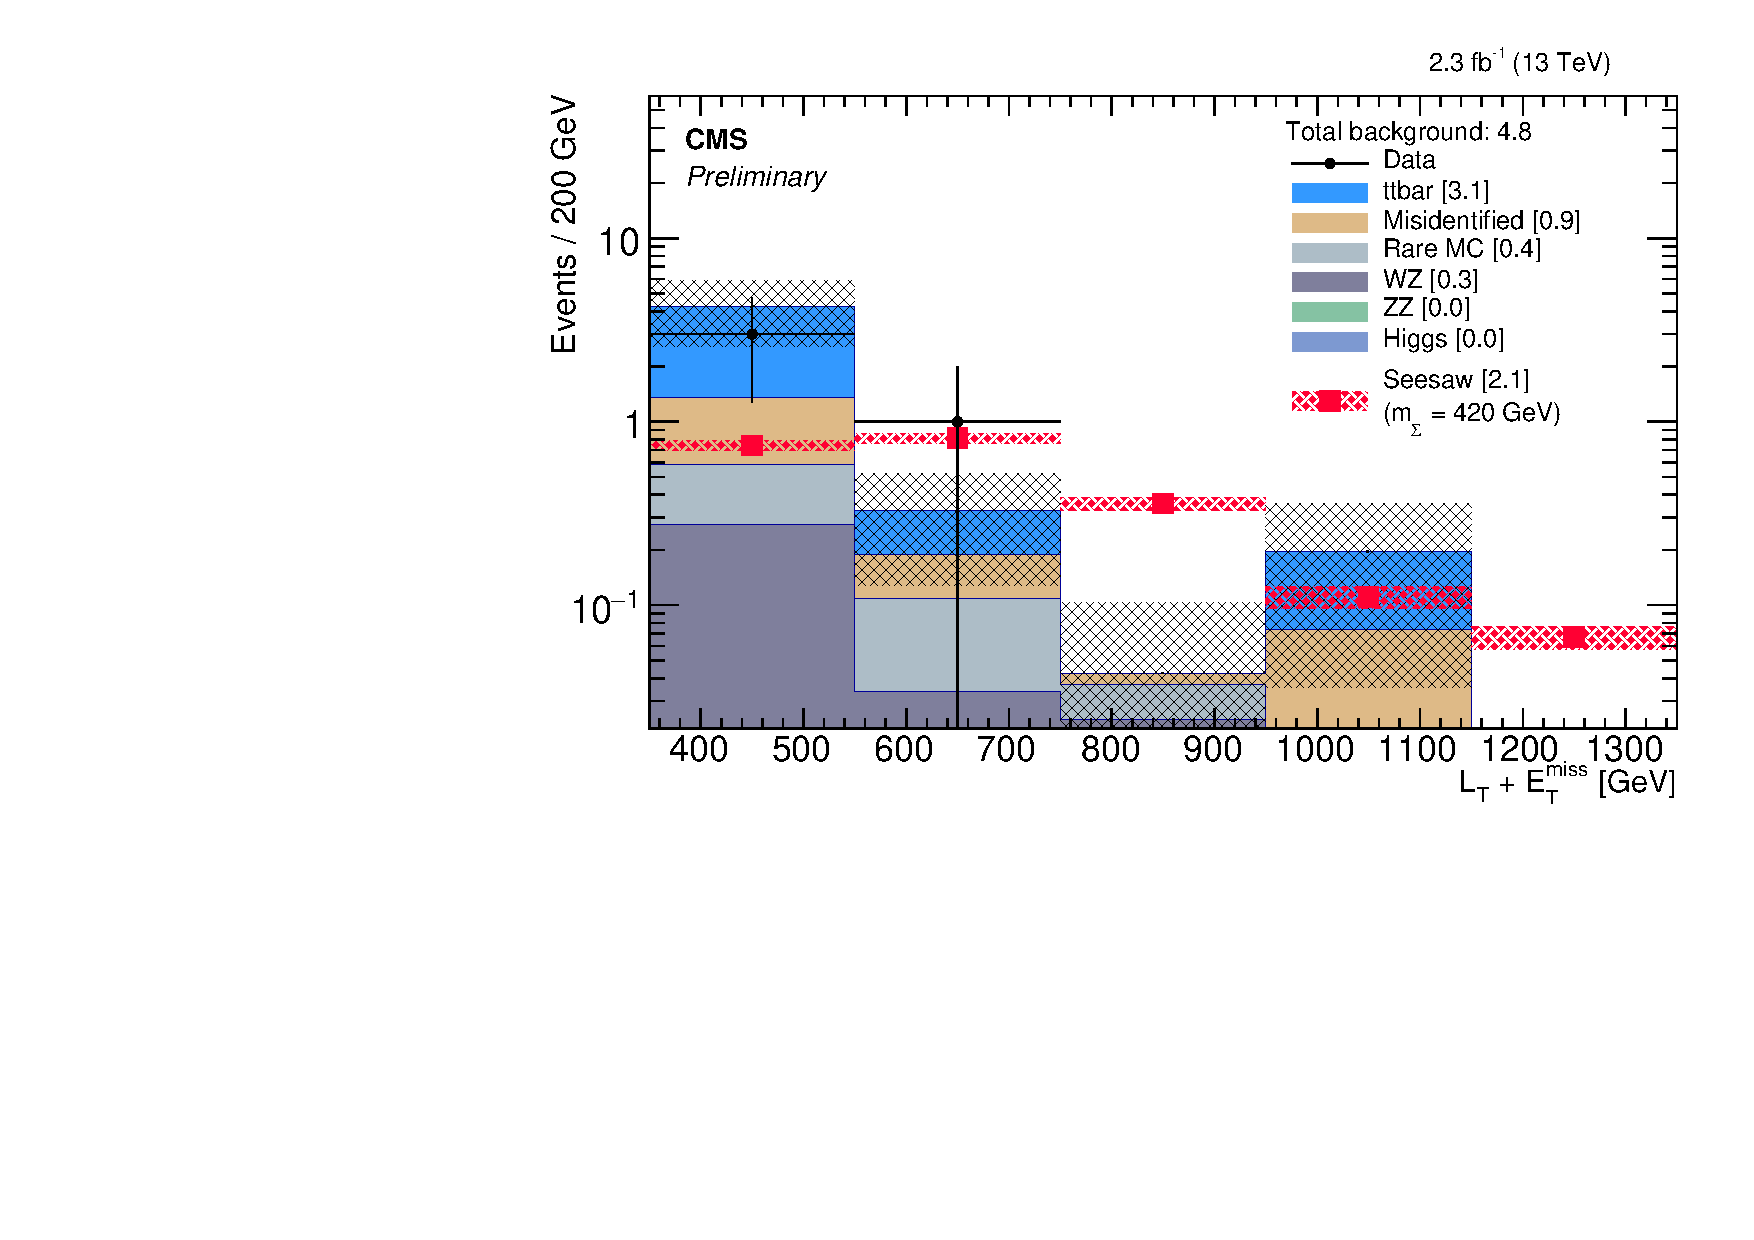
\includegraphics[width=\textwidth]{Results/plots/L3DY0}
		\caption{3 leptons, no OSSF pair}
	\end{subfigure}%
	\begin{subfigure}[b]{.5\textwidth}
		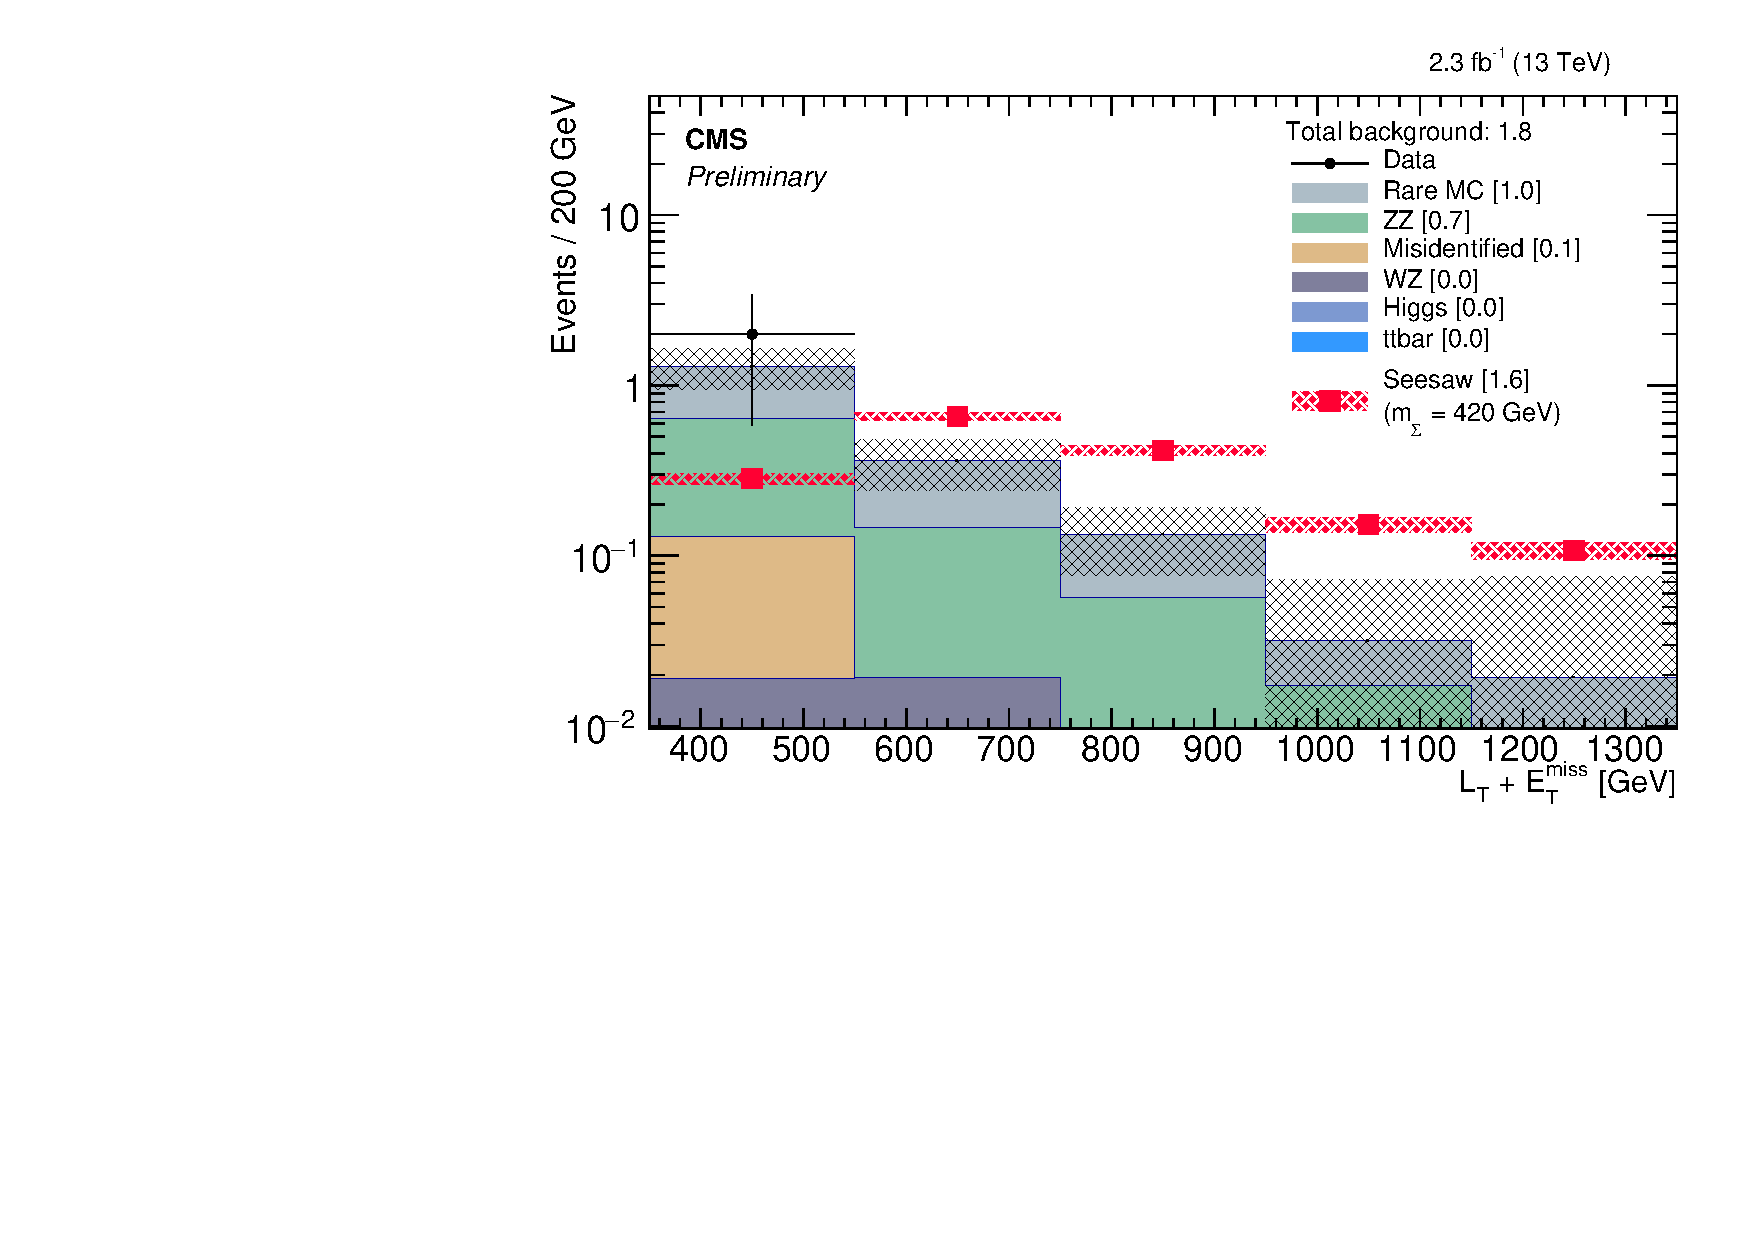
\includegraphics[width=\textwidth]{Results/plots/L4DYgt0}
		\caption{4 leptons, at least 1 OSSF pair}
	\end{subfigure}%
	\caption{Results: $L_\textrm{T} + \MET$ distributions (last bin includes overflow in all plots).
	\label{fig:Results}}
\end{center}
\end{sidewaysfigure}

The observations are generally consistent with the SM expectations, with the possible exception of the 3-lepton category that includes an OSSF lepton pair with invariant mass consistent with that of the Z boson (Fig.~\ref{fig:Results/a}). The dominant background for this category is the \WZ diboson production, as shown. Detailed investigations of the extra events did not uncover any unexpected kinematic patterns. Fig.~\ref{fig:Results/eventDisplays} presents event displays for two of the events in this category.

\begin{figure}
\begin{center}
	\begin{subfigure}{\textwidth}
		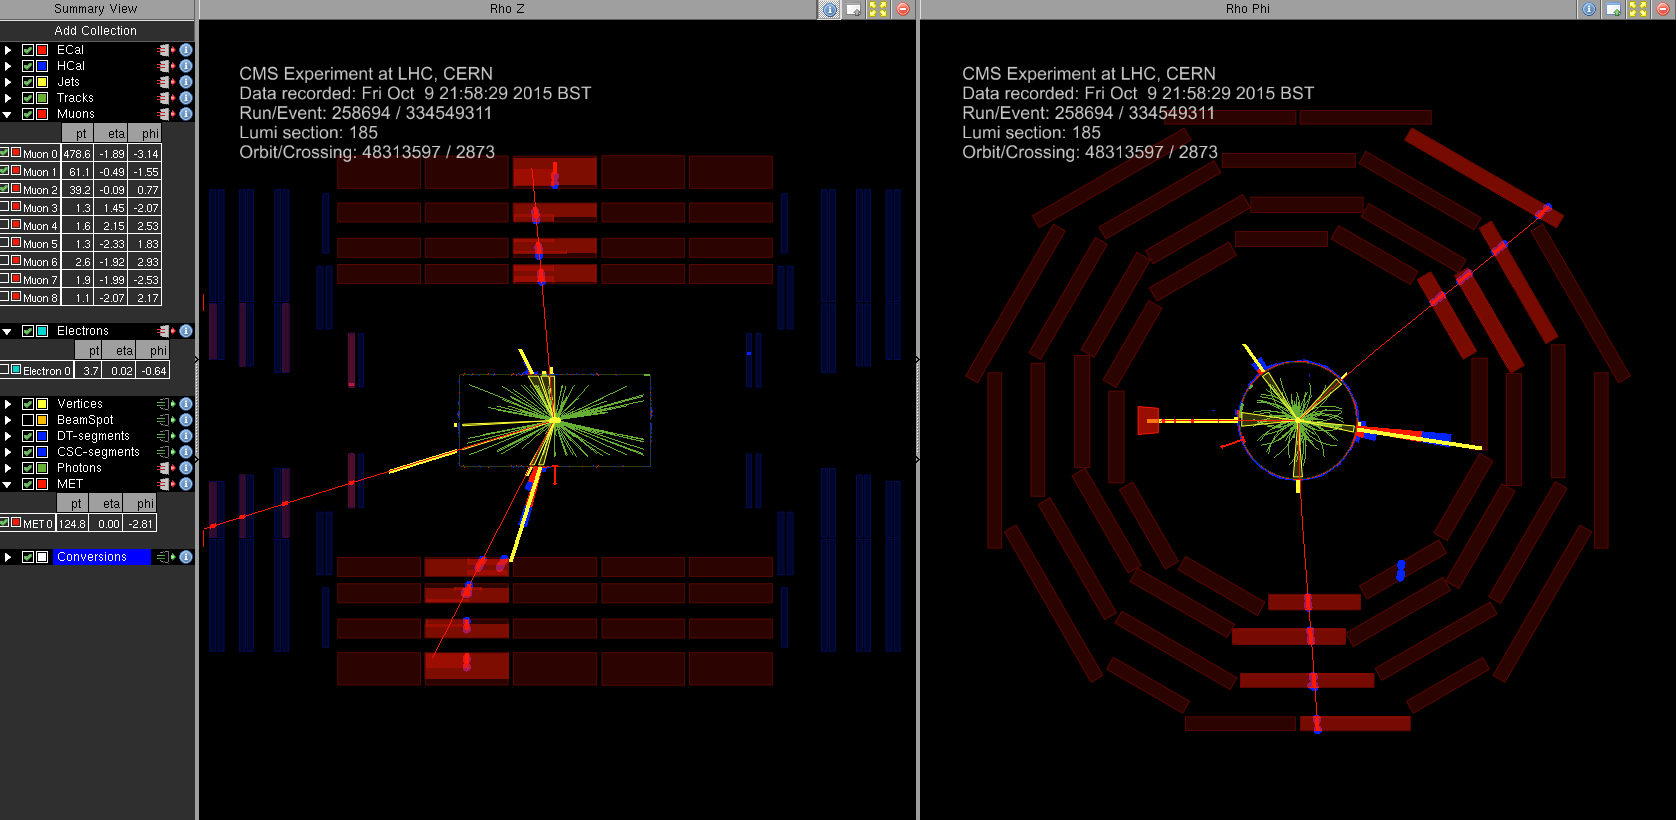
\includegraphics[width=\textwidth]{Results/EventDisplay_DoubleMuon}
		\caption{DoubleMuon-triggered event \vspace{1em}}
	\end{subfigure}
	\begin{subfigure}{\textwidth}
		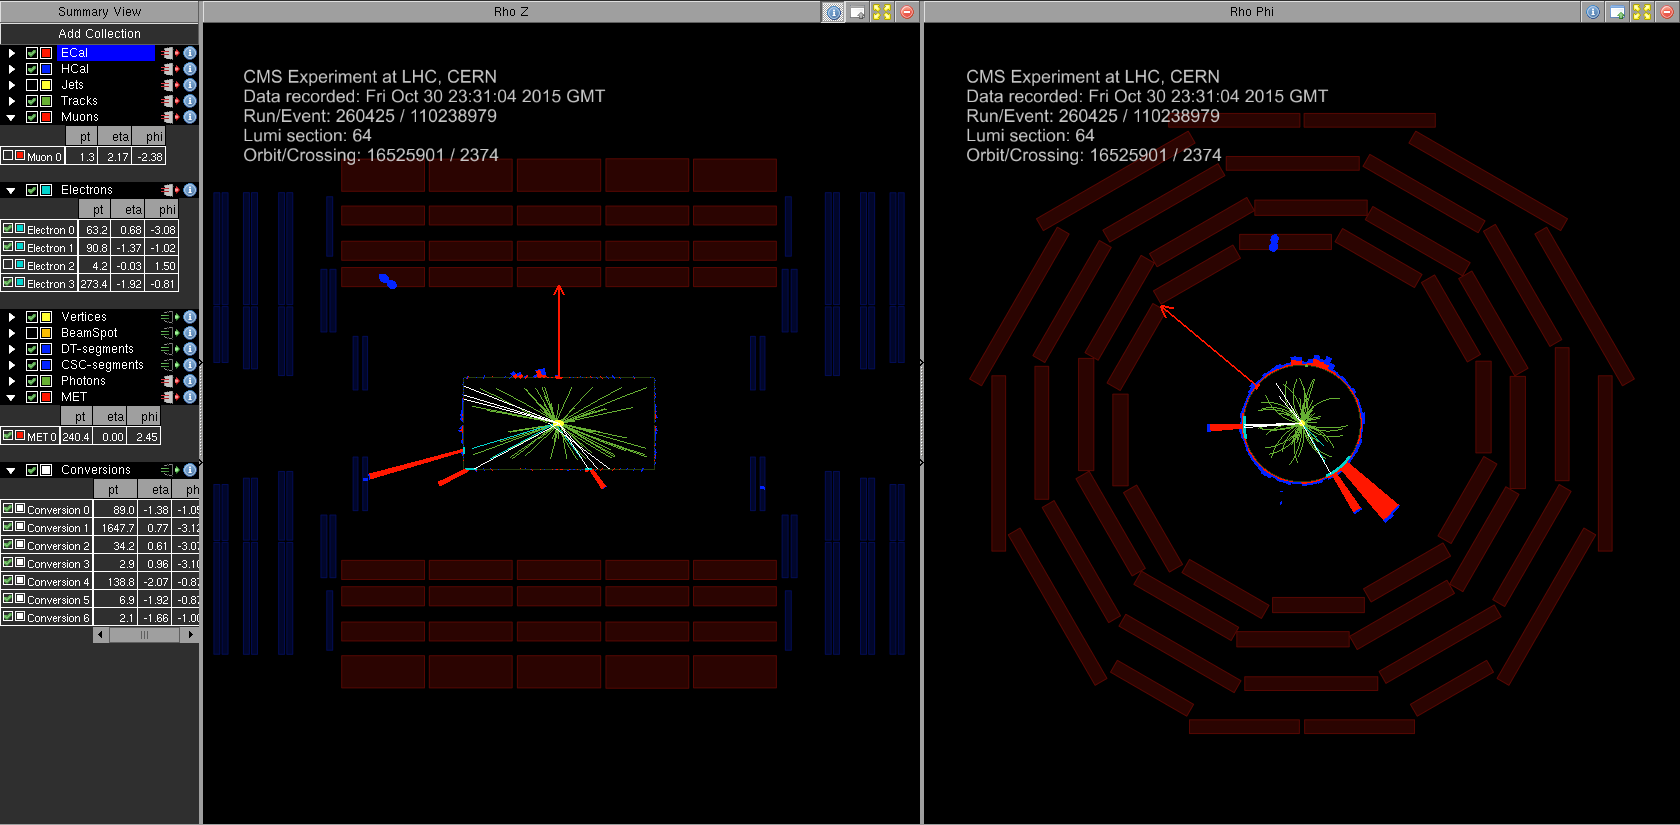
\includegraphics[width=\textwidth]{Results/EventDisplay_DoubleEG}
		\caption{DoubleEG-triggered event}
	\end{subfigure}
	\caption{Event displays for events from Fig.~\ref{fig:Results/a}.
	\label{fig:Results/eventDisplays}}
\end{center}
\end{figure}

The $p$-value for the observation in the aggregated 20 $L_\textrm{T} + \MET$ bins for the four categories shown in Fig.~\ref{fig:Results}, assuming SM physics only, is 0.93. This overall consistency with the SM expectation conveys the message that the excess of observed events in the Fig.~\ref{fig:Results/a} is either a statistical artifact or a discrepancy that can be addressed only with additional data.

\section{Interpretation for the Seesaw Model}
\label{sec:Interpretation}
\label{sec:Interpretation/Seesaw}

As no statistically significant excess was observed, we calculate expected and observed upper limits on the cross section sum for the production of seesaw heavy fermion pairs ($\Sigma^0\Sigma^+$, $\Sigma^0\Sigma^-$, or $\Sigma^+\Sigma^-$), assuming a flavor-democratic value for the mixing angle parameters, $V_e = V_\mu = V_\tau = 10^{-6}$, and degenerate heavy fermion masses $m_\Sigma$.

By comparing with the signal production cross section, one can translate the cross section limits into limits on the heavy fermion mass which can be excluded based on the data. In particular, taking $r$ to be the ratio of the cross section limit and the signal production cross section, we can exclude the signal hypothesis when $r < 1$.
The calculation is done using asymptotic CL$_s$ limits with a confidence level of 95\,\% \cite{Junk:1999kv,Read:2000ru,Read:2002hq}.
%Taking the ratio of the cross section upper limit and the signal cross section, one obtains the so-called $r$-value which indicates whether the signal at hand is excluded ($r < 1$) or cannot be excluded ($r > 1$).

\subsection{Single-channel Limits}
\label{sec:Results/singleChannel}

We first compute limits for the 10 most sensitive of the bins displayed in Fig.~\ref{fig:Results}. To get a feeling on how different signal regions contribute to the limits presented in Sec.~\ref{sec:Interpretation}, we present the expected single-channel $r$-values for these top 10 channels in Table~\ref{tab:topSensitivity}, using the signal hypothesis with $m_\Sigma = 420\GeV$.

\begin{table}
\centering
\caption{Relative Sensitivity of Signal Regions.} \label{tab:topSensitivity}
%\caption*{DY0: no OSSF pair, DYz1: 1 pair on \Z,\\ DYh1: 1 pair above \Z, DYgt0: $\geq 1$ pair}
\begin{tabular}{cccc}
\hline\hline
$n_\textrm{leptons}$ & OSSF pair & $L_\textrm{T} + \MET$ [GeV] & $r_\textrm{exp}$\\
\hline
3        & above-\Z & 550--750 & 2.6953\\
3        & none     & 550--750 & 3.6094\\
3        & above-\Z & 750--950 & 4.0781\\
$\geq 4$ & n/a      & 550--750 & 4.1094\\
$\geq 4$ & n/a      & 750--950 & 5.5938\\
\hline
3        & none     & 750--950 & 5.8750\\
3        & above-\Z & 350--550 & 6.2500\\
3        & on-\Z    & 550--750 & 6.7188\\
3        & none     & 350--550 & 7.5938\\
3        & above-\Z & 950--1150 & 8.7812\\
\end{tabular}
\end{table}

As can be seen from the table, no single signal bin is sensitive enough to exclude the signal hypothesis; still, the table presents the relative sensitivities. However, we show below that the combination of several of these channels is sensitive enough to exclude a considerable range of the signal mass parameter.

\subsection{Multi-channel Limits}
Fig.~\ref{fig:exclusions} shows the mass limits for each of the categories presented in Fig.~\ref{fig:Results}. It can be seen that the observed limit is better, i.\,e. lower, than the expected limit whenever there is a deficiency observed in data. Similary, when the data is high, the observed limit is worse than expected. This is the case in particular for the observed limit in Fig.~\ref{fig:exclusions/a}, as there is an excess of events in the corresponding signal region (Fig.~\ref{fig:Results/a}). However, the impact of this excess on the overall result is limited, as this particular signal region is not very sensitive to the type-III seesaw signal and thus yields cross section limits that are much higher than those of the other signal regions limits (see also Sec.~\ref{sec:Results/singleChannel}). This can also be seen by the fact that this signal region is the only one that is not sensitive enough to exclude any of the masses probed, while the other signal regions achieve mass limits between 300 and 380\GeV on their own. (Masses to the left of the intersection point are excluded.)

\begin{sidewaysfigure}
\begin{center}
	\begin{subfigure}[b]{.5\textwidth}
		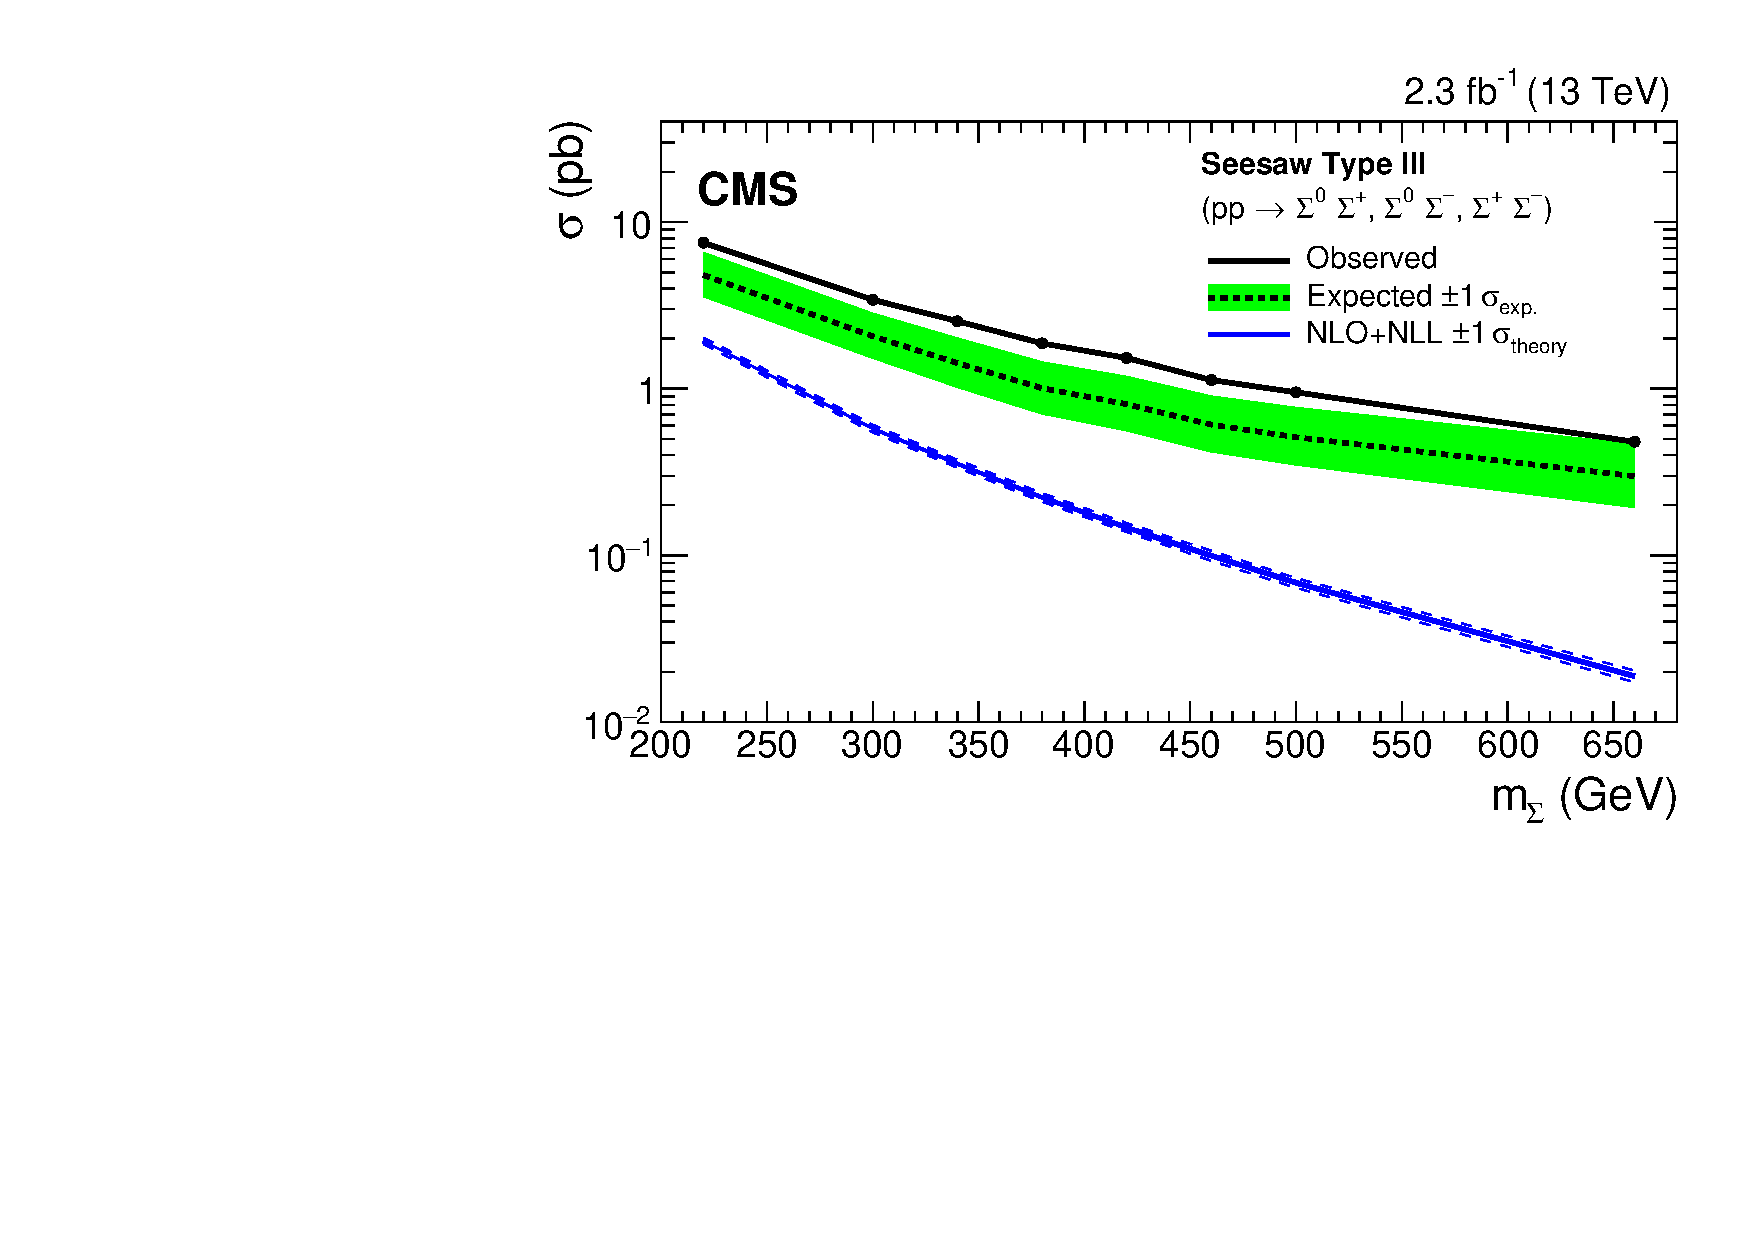
\includegraphics[width=\textwidth]{Results/exclusion-L3DYz1}
		\caption{3 leptons with OSSF pair on-\Z} \label{fig:exclusions/a}
	\end{subfigure}%
	\begin{subfigure}[b]{.5\textwidth}
		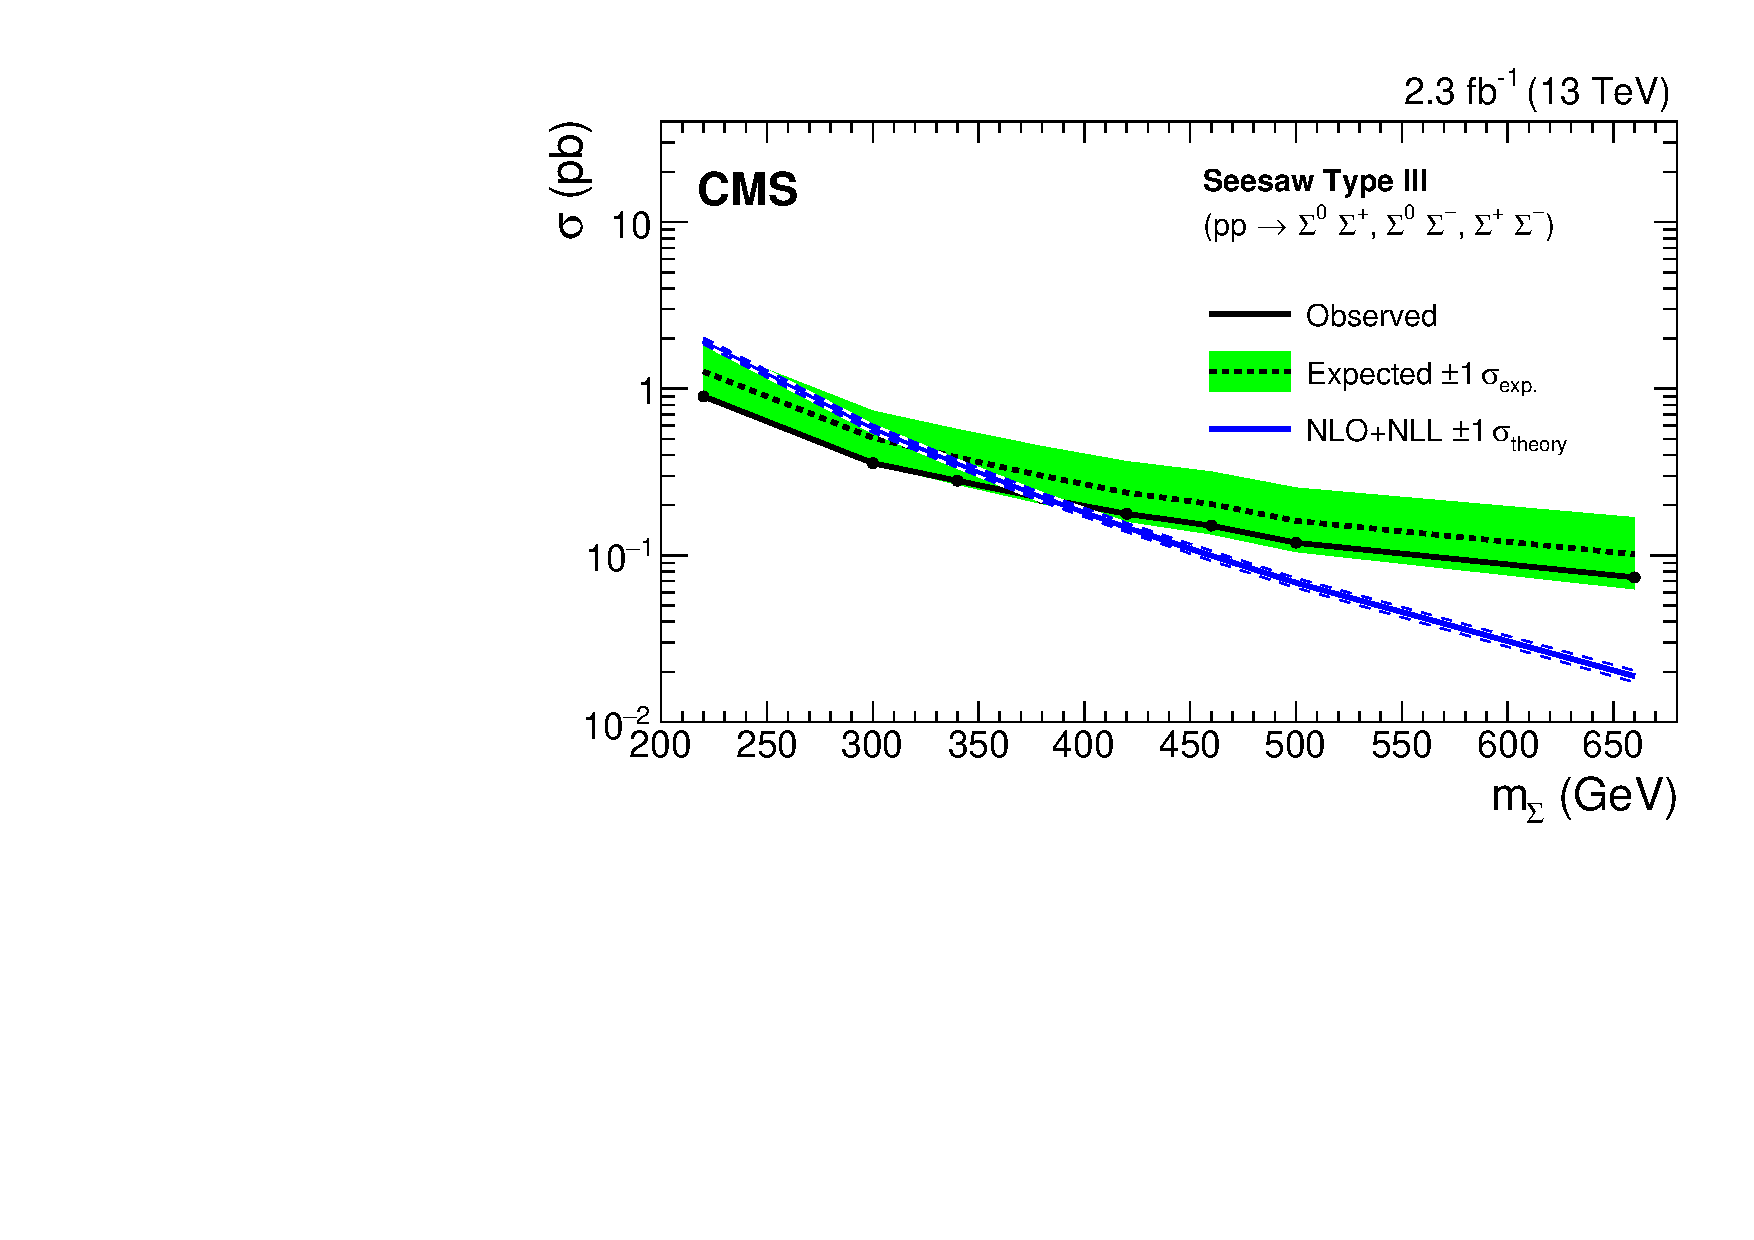
\includegraphics[width=\textwidth]{Results/exclusion-L3DYh1}
		\caption{3 leptons with OSSF pair above-\Z}
	\end{subfigure}
	\begin{subfigure}[b]{.5\textwidth}
		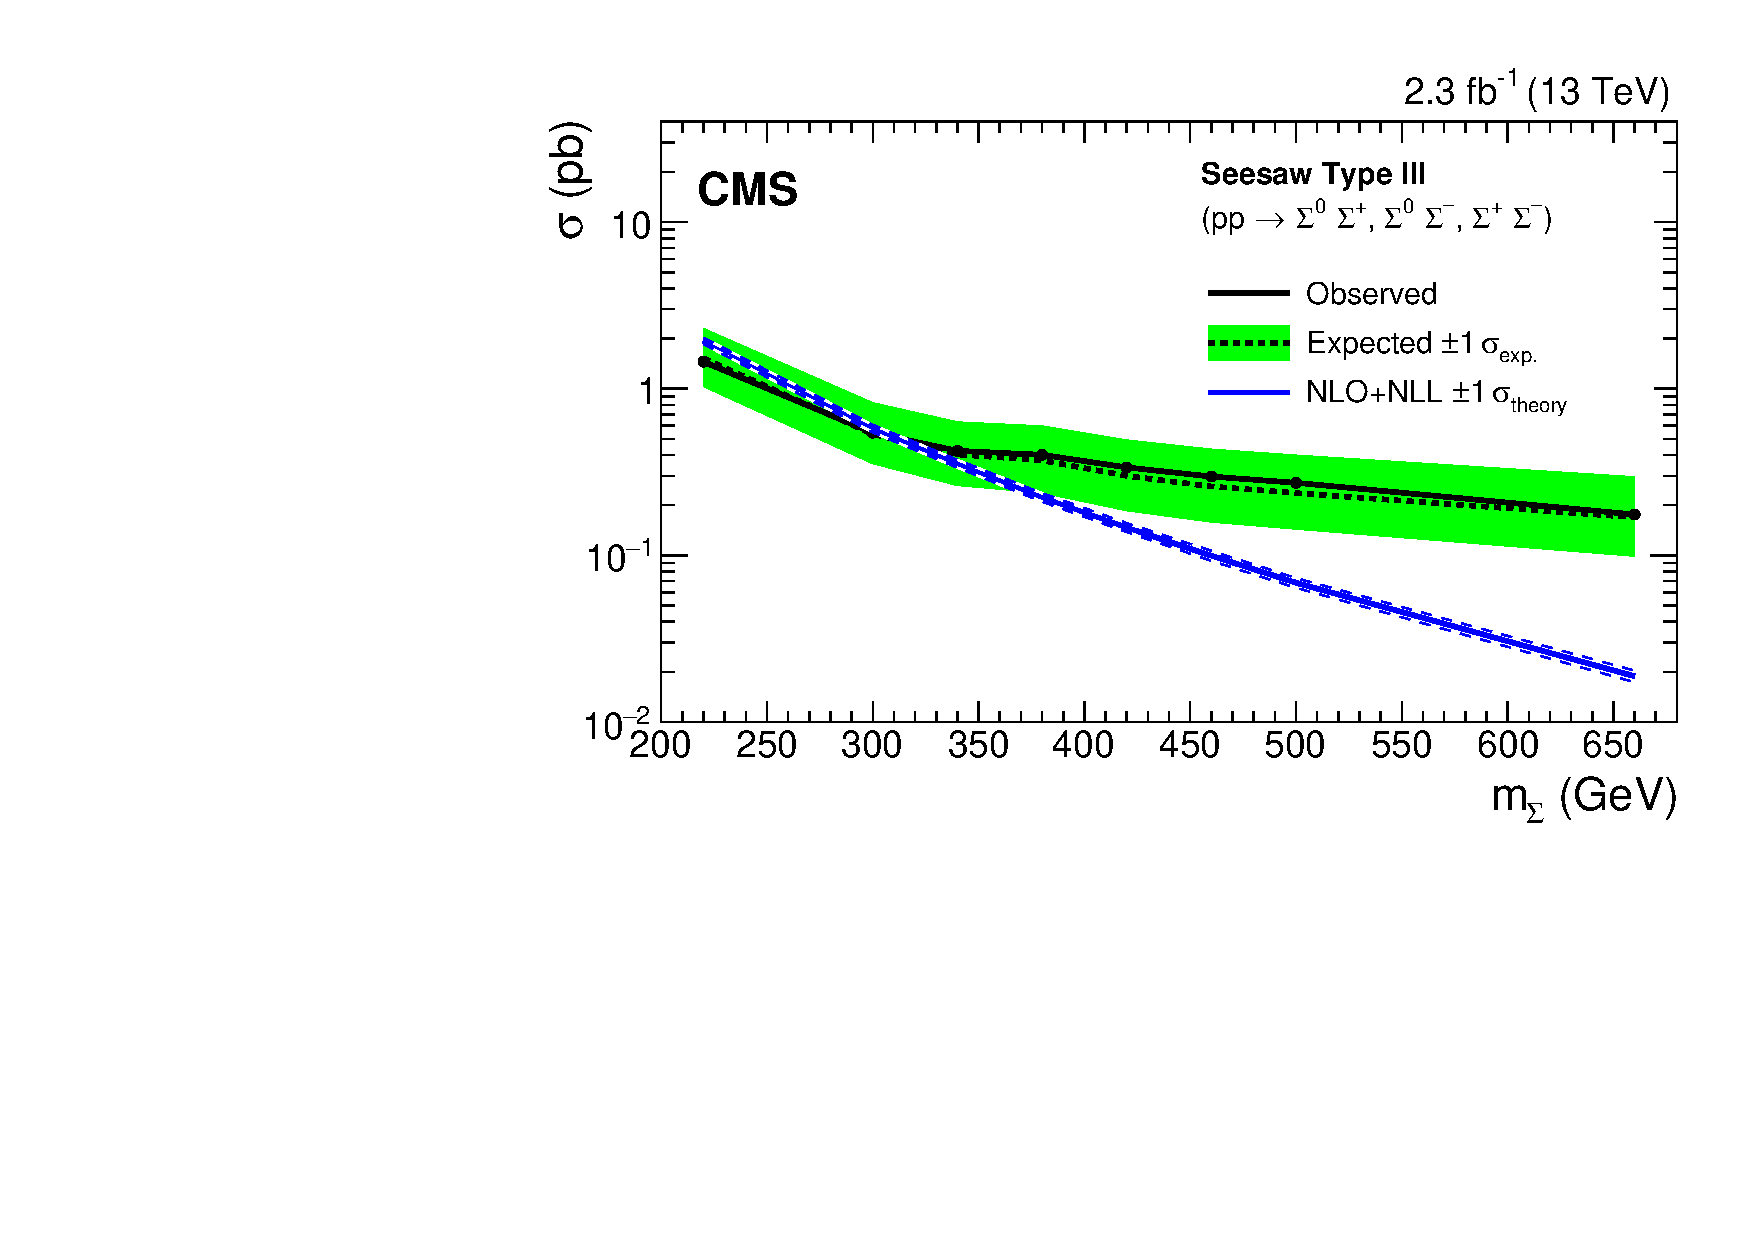
\includegraphics[width=\textwidth]{Results/exclusion-L3DY0}
		\caption{3 leptons, no OSSF pair}
	\end{subfigure}%
	\begin{subfigure}[b]{.5\textwidth}
		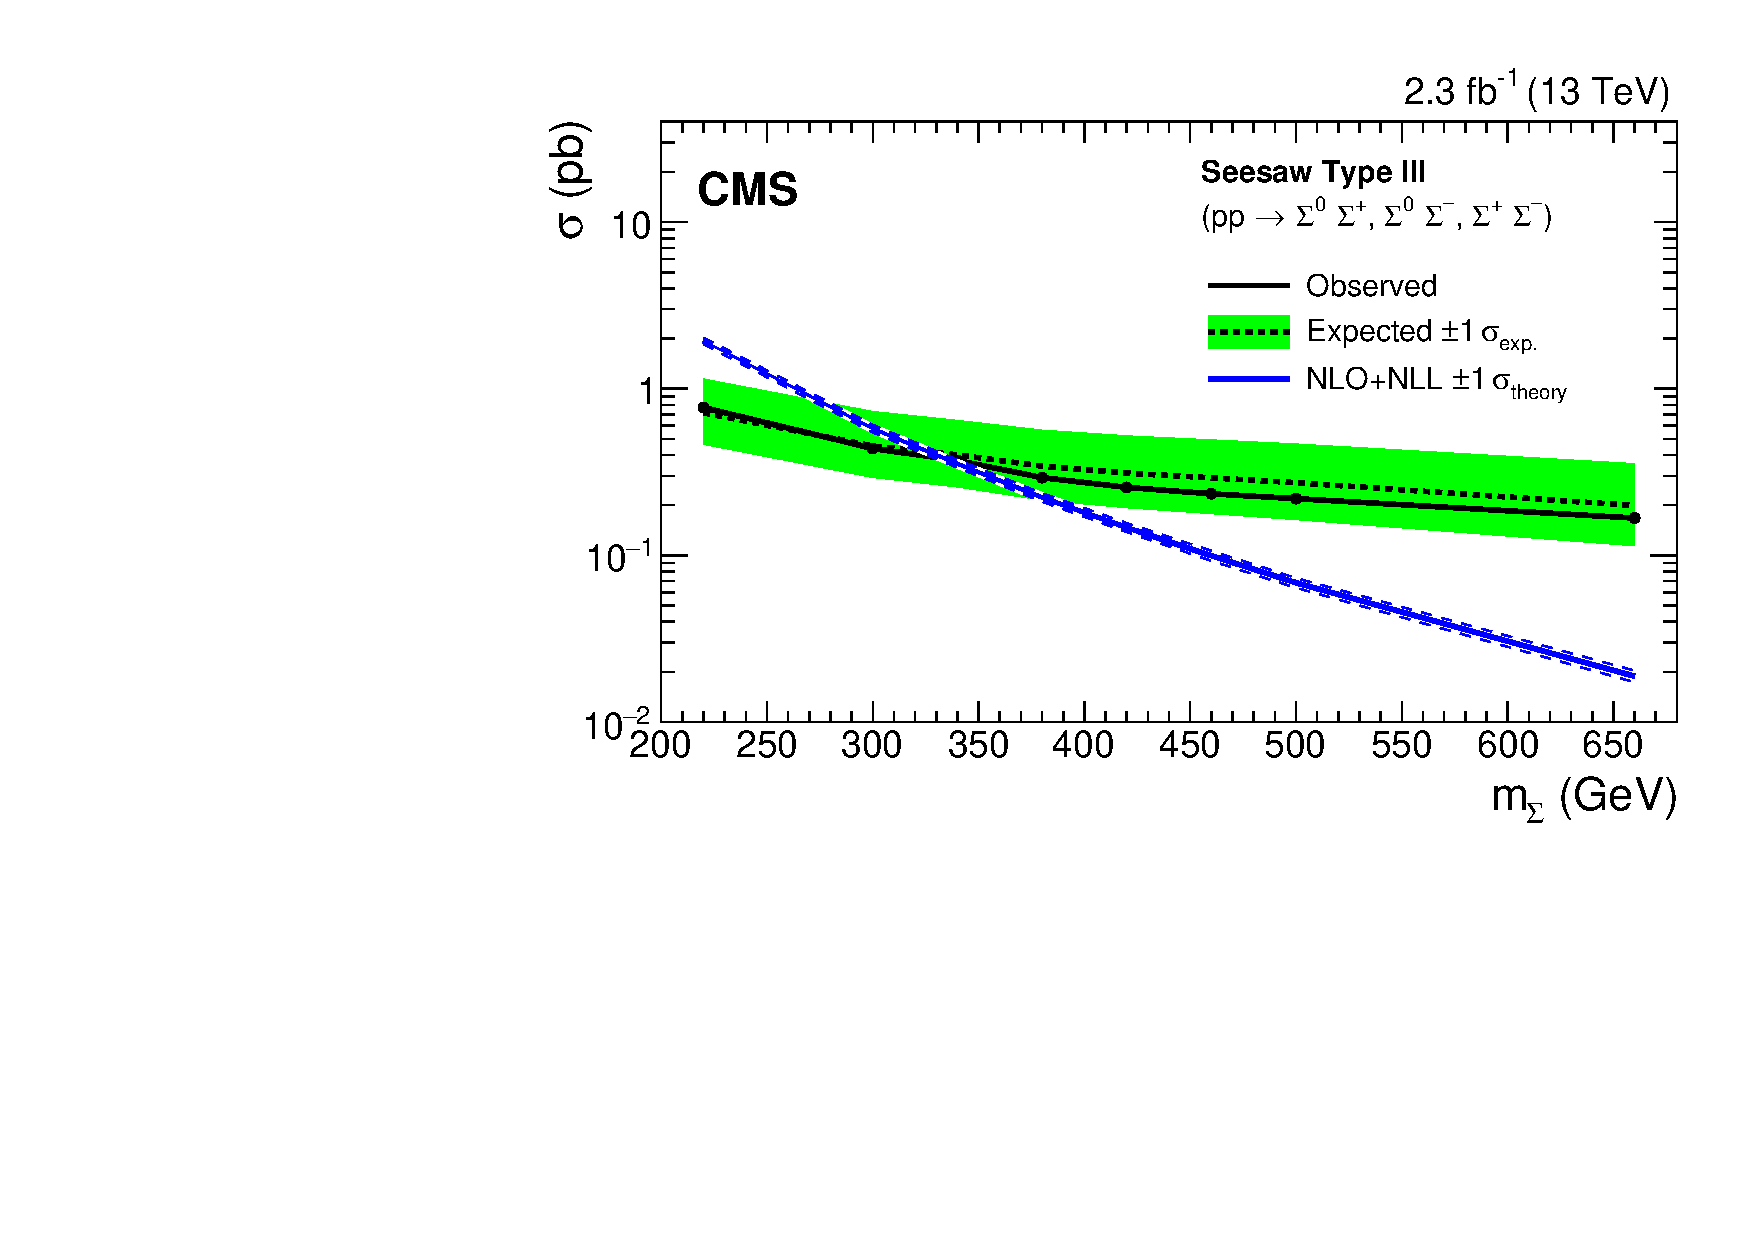
\includegraphics[width=\textwidth]{Results/exclusion-L4DYgt0}
		\caption{4 leptons, at least 1 OSSF pair}
	\end{subfigure}%
	\caption{Results: Exclusion curves. Masses to the left of the intersection point are excluded.
	\label{fig:exclusions}}
\end{center}
\end{sidewaysfigure}

\subsection{Full Combination}
If the data agreed perfectly with the background estimates in all signal regions combined, we would expect our analysis to exclude type-III seesaw heavy fermion pair production for masses below $m_\Sigma = 430\GeV$. The combined observed limit is at 440\GeV. The full exclusion curve is shown in Fig.~\ref{fig:exclusion}.

\begin{figure}
\begin{center}
	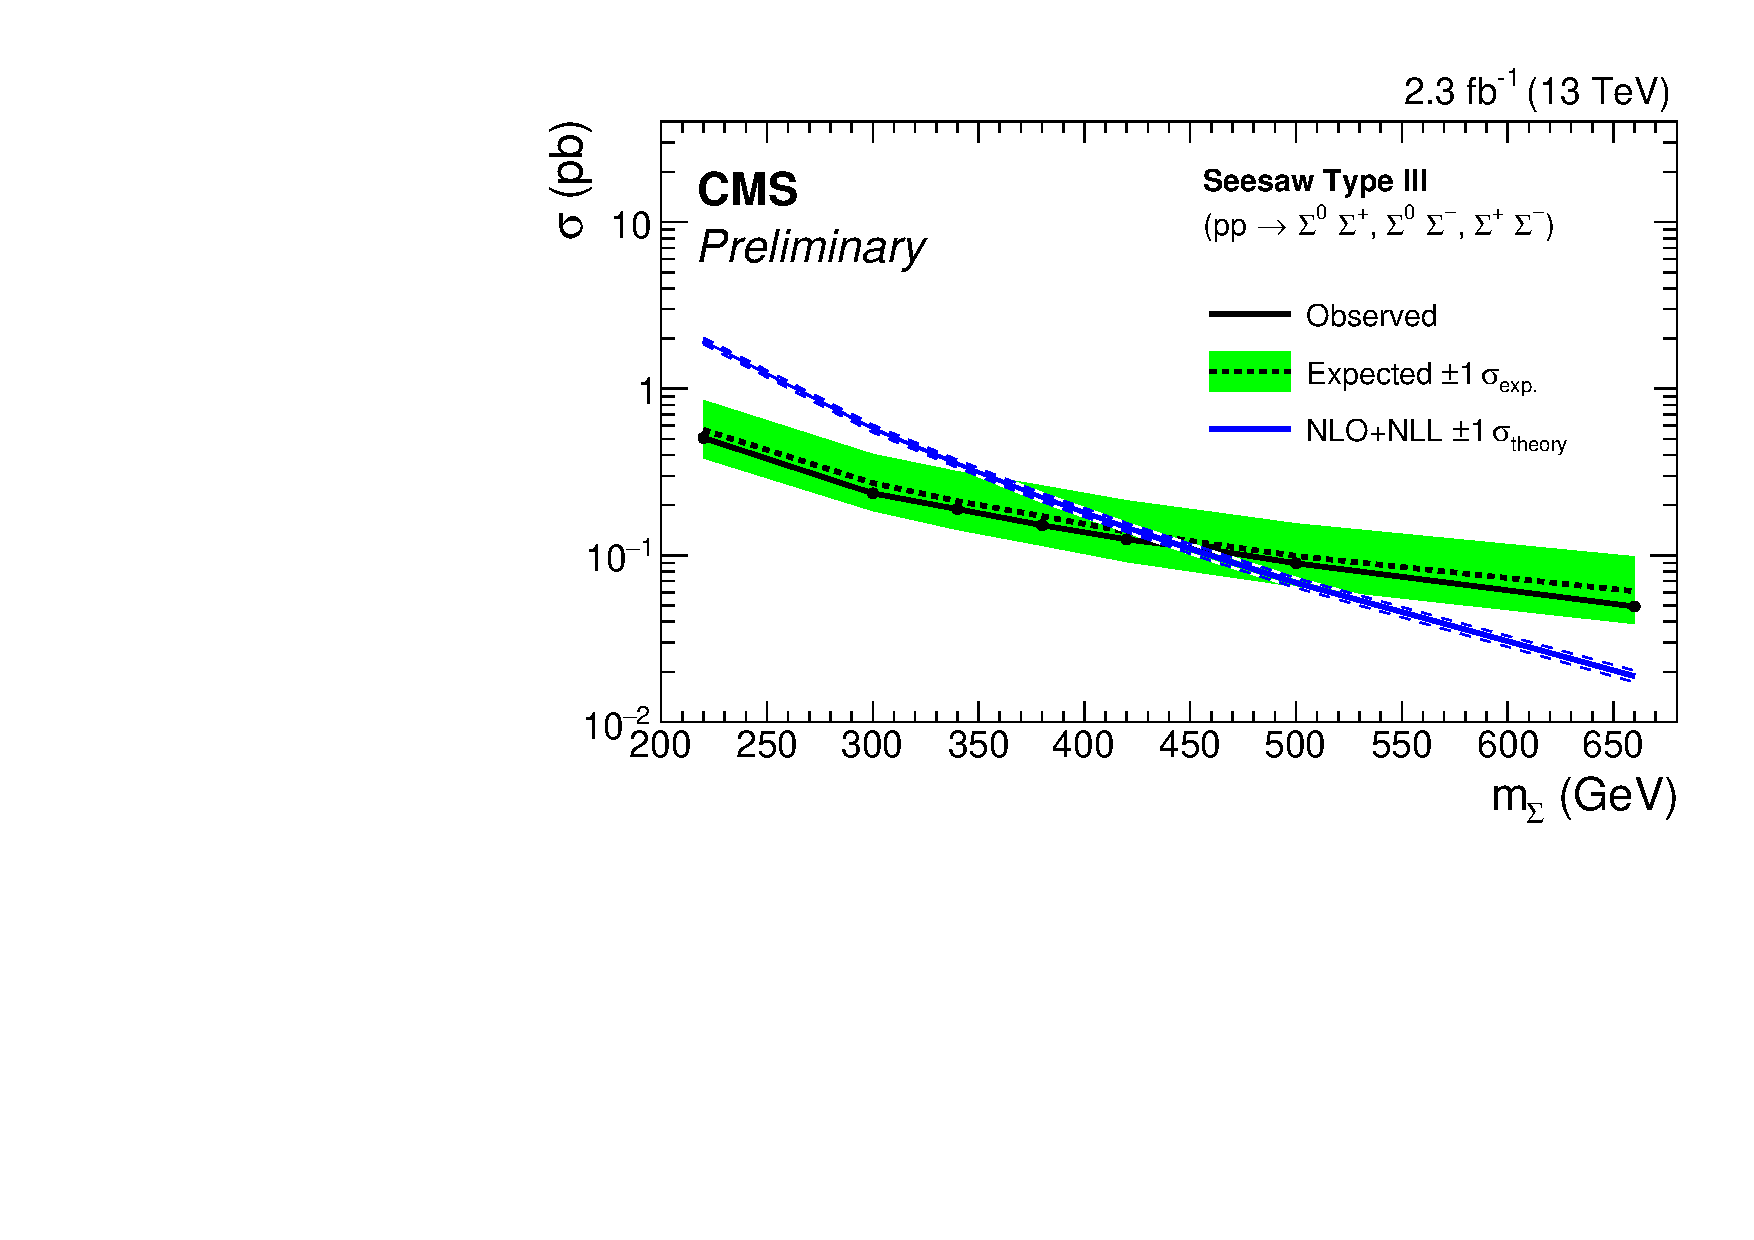
\includegraphics[width=.8\textwidth]{Results/exclusion}
	\caption{Exclusion for the flavor-democratic type-III seesaw model ($V_e = V_\mu = V_\tau = 10^{-6}$). We exclude heavy fermion pair production for masses below $m_\Sigma = 440\GeV$ (expected: 430\GeV) and give upper limits on the pair production cross section.
	\label{fig:exclusion}}
\end{center}
\end{figure}

In comparison to the Run-I results, the search sensitivity has been enhanced by various improvements, most notably the inclusion of new decay modes involving the Higgs boson and of 4-lepton channels, as well as by the introduction of an improved fine-grained binning scheme. Exclusion limits from the CMS Run I result were at $m_\Sigma = 250\GeV$ (expected) and $m_\Sigma = 278\GeV$ (observed) \cite{CMS-PAS-EXO-14-001}.

\section{Cross-checks}
\subsection{Back-of-the-Envelope Limits}
\label{sec:Results/BackOfEnvelope}
We derive a rough estimate of the $r$-values for the $m_\Sigma = 220\GeV$ mass point manually to verify that our result from Sec.~\ref{sec:Interpretation} is in the right ballpark. The relatively low mass was chosen so that we obtain a sizeable number of expected signal events. We consider 4 groups of processes:
\begin{itemize}
	\item $(\Sigma^\pm, \Sigma^0) \to (\PW^\pm \nu, \PW^\pm \ell^\mp)$
	\item $(\Sigma^\pm, \Sigma^0) \to (\Z \ell^\pm, \PW^\pm \ell^\mp)$
	\item $(\Sigma^\pm, \Sigma^0) \to (\PH \ell^\pm, \PW^\pm \ell^\mp)$
	\item $(\Sigma^+, \Sigma^-) \to (\Z \ell^+, \Z \ell^-)$
\end{itemize}
These are the production and decay modes amongst the 27 combinations described in Sec.~\ref{sec:Theory/SeesawPhenomenology} that have the highest branching ratios to trilepton final states. Note that in the first three cases, we sum over the heavy fermion charges, so that the above list covers seven of the 27 processes.

We first estimate the expected number of decays from each of these processes, based on which we calculate how many of these events we expect to reconstruct and select in our analysis. We then compute back-of-the-envelope limits for a simplified search channel with exactly three light leptons\footnote{We apply an AIC veto to reject events with an OSSF pair below \Z when the trilepton invariant mass is on \Z (see Sec.~\ref{sec:bkg_fakeLight/photons}).}.

To calculate the expected number of decays to the bosonic level from the most significant processes, we compute the product of the cross section and branching ratio for each process and then multiply by the luminosity (\fullLumi) as shown in Table~\ref{tab:BackOfEnvelope/1}.

\begin{table}
\centering
\caption{Most significant trilepton processes with branching ratios to the bosonic level.} \label{tab:BackOfEnvelope/1}
\begin{tabular}{lcc}
\hline\hline
Process                                                       & $\sigma \cdot \textrm{BR}$ [fb] & $N = \sigma \cdot \textrm{BR} \cdot \mathcal{L}$ \\
\hline
$(\Sigma^\pm, \Sigma^0) \to (\PW^\pm \nu, \PW^\pm \ell^\mp)$  & 418                             & 961 \\
$(\Sigma^\pm, \Sigma^0) \to (\Z \ell^\pm, \PW^\pm \ell^\mp)$  & 202                             & 465 \\
$(\Sigma^\pm, \Sigma^0) \to (\PH \ell^\pm, \PW^\pm \ell^\mp)$ & 100                             & 230 \\
$(\Sigma^+, \Sigma^-) \to (\Z \ell^+, \Z \ell^-)$             & 49                              & 113 \\
\end{tabular}
\end{table}

To obtain the expected number of reconstructed signal events, the number of expected decays then needs to be multiplied by the branching fractions from the bosonic to the leptonic level. We use $\textrm{BR}(\PW \to e \text{ or } \mu) = 23\,\%$, $\textrm{BR}(\Z \to e \text{ or } \mu) = 16\,\%$, as well as $\textrm{BR}(\ell\to e \text{ or } \mu) = 72\,\%$ to take leptonic $\tau$ decays into account. Whenever a \PW\ boson is present, it has a much higher leptonic branching ratio than the Higgs or \Z bosons which may also be present. Furthermore, there are two prompt leptons from the heavy fermion decay. In the presence of a \PW\ boson, we therefore ignore any Higgs and \Z bosons for simplicity. The electron and muon reconstruction efficiency is taken at $\epsilon_\textrm{lep} = 83\,\%$. Table~\ref{tab:BackOfEnvelope/2} shows the event yields with these branching ratios and efficiencies taken into account. As can be seen in the table, a total of about 74 signal events is expected. 

\begin{table}
\centering
\caption{Estimate of reconstructed trilepton signal events. The combined leptonic branching ratio of all involved bosons is denoted as $\textrm{BR}_\textrm{lep}$.} \label{tab:BackOfEnvelope/2}
\begin{tabular}{lccc}
\hline\hline
Process & $N \cdot \textrm{BR}_\textrm{lep}$ & $N \cdot \textrm{BR}_\textrm{lep} \cdot \epsilon_\textrm{lep}^3$ & Exact yield from full analysis \\
\hline
$(\Sigma^\pm, \Sigma^0) \to (\PW^\pm \nu, \PW^\pm \ell^\mp)$  & 36.6 & 20.9 & 13.9 \\ % $23\% \cdot 23\% \cdot 72\%$ & 
$(\Sigma^\pm, \Sigma^0) \to (\Z \ell^\pm, \PW^\pm \ell^\mp)$  & 55.4 & 31.7 & 35.9 \\ % $72\% \cdot 72\% \cdot 23\%$ & 
$(\Sigma^\pm, \Sigma^0) \to (\PH \ell^\pm, \PW^\pm \ell^\mp)$ & 27.4 & 15.7 & 19.2 \\ % $72\% \cdot 72\% \cdot 23\%$ & 
$(\Sigma^+, \Sigma^-) \to (\Z \ell^+, \Z \ell^-)$             & 9.4  & 5.4  & 5.7  \\ % $16\% \cdot 72\% \cdot 72\%$ & 
\hline
Sum               & 128.8                & 73.7              & 74.7 \\
\end{tabular}
\end{table}

We now consider the total background for three light leptons, only applying the lepton \pt thresholds (see Sec.~\ref{sec:Selection}) and the AIC veto. We find about 2000 events, based on which we can set a 95\,\% C.\,L. limit of about $3 \cdot \sqrt{2000} \approx 134$ events. Relating this to the expected signal yields $r = \frac{74}{134} = 0.55$.

This number is larger by a factor of 1.9 than our main result at 220\GeV, indicating that our estimate has less sensitivity. The reason for this is that we did not use any kinematic binning to separate the signal from the background. Thus, the limit is worse, as expected, but not vastly off.

\subsection{Simplified Limits from Leading Production and Decay Modes}
The seven signal production and decay modes considered in \ref{sec:Results/BackOfEnvelope} are responsible for the bulk of the detectable signal yield. Other modes contribute little due to small branching ratios to multilepton final states. We study what the limit would be if we only used these seven modes, and present the corresponding exclusion plot in Fig.~\ref{fig:exclusion-leading7}.

While this exclusion plot visually differs little from the main result (Fig.~\ref{fig:exclusion}), the degradation of the cross section limit value at 400\GeV is still 25\,\%, worsening the expected mass limit by about 45\GeV. This indicates that although the remaining 22 modes are of secondary importance, they should not be fully ignored.

\begin{figure}
\begin{center}
	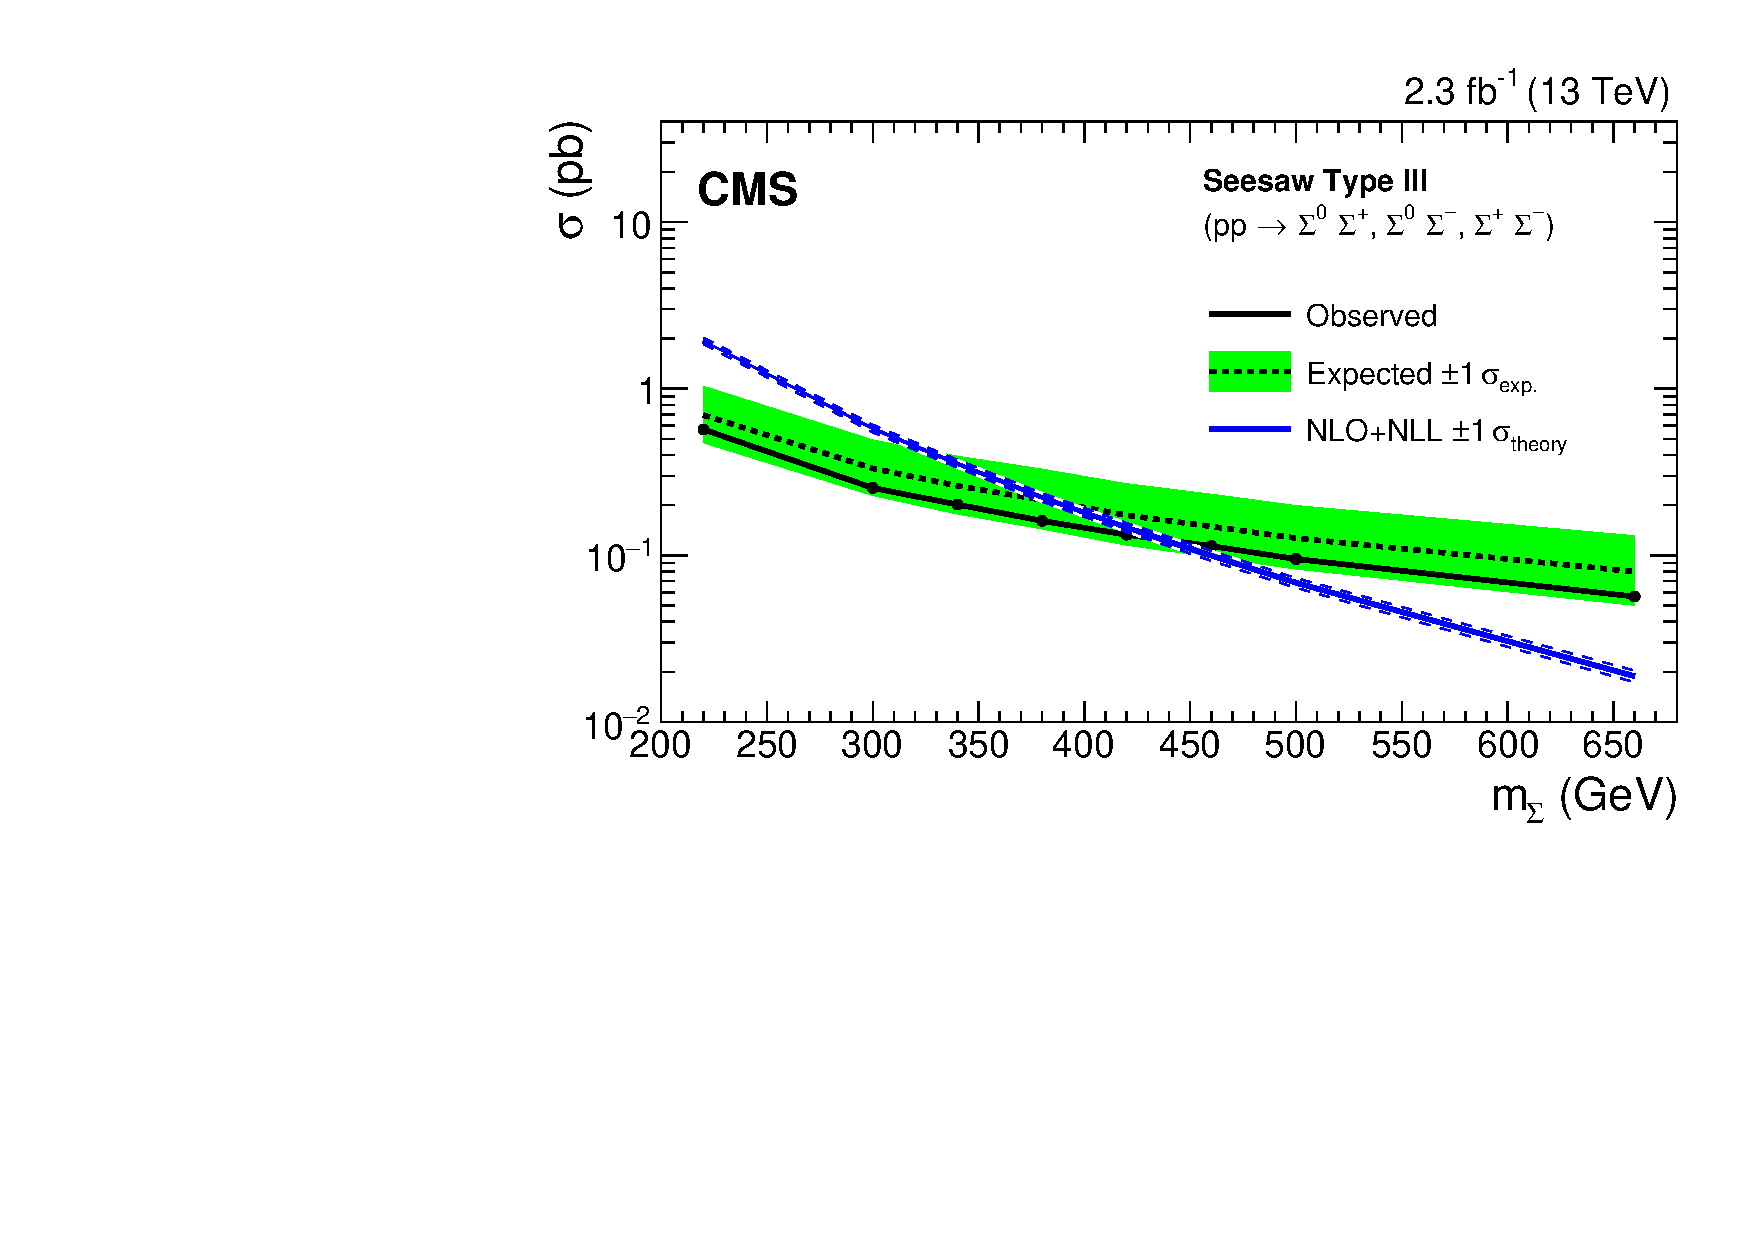
\includegraphics[width=.8\textwidth]{Results/exclusion-leading7}
	\caption{Exclusion for the flavor-democratic type-III seesaw model using the seven leading signal production/decay modes only.
	\label{fig:exclusion-leading7}}
\end{center}
\end{figure}

\subsection{Comparison to Run-I Results}
We show that the sensitivity of our current analysis is plausible, given the improvements that were made in comparison to the Run I analysis \cite{CMS-PAS-EXO-14-001}. To this end, we compute expected limits starting from a mock-up analysis setup that is very similar to the Run I analysis. As we then add various improvements, we arrive at the limit shown in Section~\ref{sec:Interpretation}. The investigations are done using the highest signal mass point considered in the Run I analysis ($m_\Sigma = 340\GeV$) and described in the following; a summary is presented in Table~\ref{tab:improvements}.

We extract the Run I expected $r$-value from Figure 2 in \cite{CMS-PAS-EXO-14-001}. We find $\frac{\sigma_\textrm{experimental} \cdot \textrm{BR}}{\sigma_\textrm{theory} \cdot \textrm{BR}} = \frac{14\,\textrm{fb}}{4.3\,\textrm{fb}} = 3.26$. To relate this 8\TeV number to the current 13\TeV dataset with 2.3\fbinv, we divide the $r$-value by the cross-section ratio $\frac{\sigma(13\TeV)}{\sigma(8\TeV)} = 3.10$ and multiply by a correction factor for the different luminosities, $\sqrt{19.5/2.3}$. We thus find that the Run I analysis sensitivity corresponds to an expected r-value of $r_\textrm{exp} = 3.06$ at 13\TeV.

Using a mock-up Run I analysis setup based on charge binning with the 13\TeV dataset (2.3\fbinv), we actually find an expected r-value of $r_\textrm{exp} = 4.11$ (exactly 3 electrons or muons, \pt thresholds at 30/20/20\GeV, $\MET > 50\GeV$, $\HT < 150\GeV$, \Z veto, AIC veto). The two charge bins that this limit is based on are displayed in Fig.~\ref{fig:app:RunI}.

4.11 is worse than 3.06 by 34\,\% which is roughly the size of the uncertainty. Furthermore, the various approximations we made to mimic the Run I analysis may cause such a difference. Also, the Run I analysis used somewhat finer flavor-dependent binning scheme. In any case, the discrepancy is in the conservative direction.

\begin{figure}
\begin{center}
	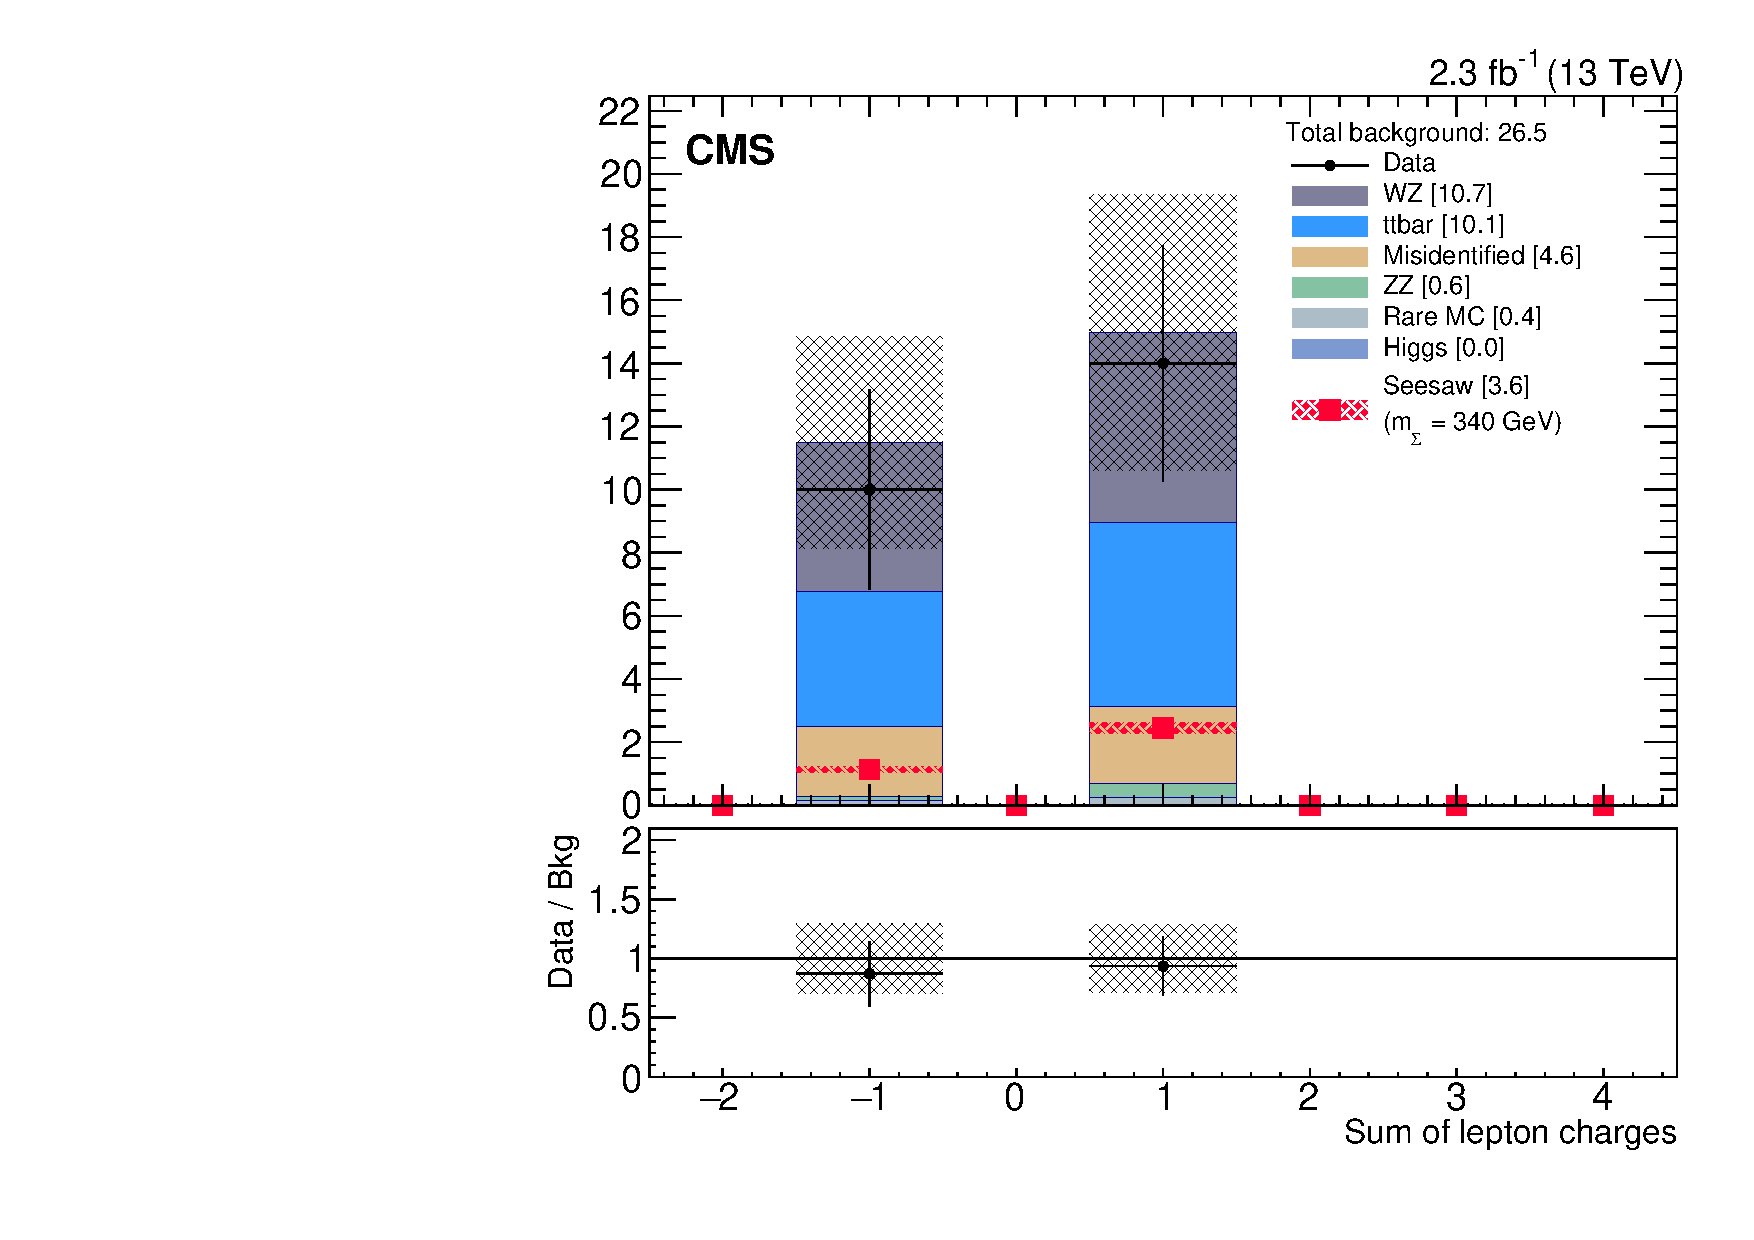
\includegraphics[width=.7\textwidth]{Results/L3Tau0_Q}\
	\caption{Bins of lepton charge sum used in mock-up Run I result, with 13\TeV dataset and background estimates (3 leptons only).
	\label{fig:app:RunI}}
\end{center}
\end{figure}

Now, starting from $r_\textrm{exp} = 4.11$, we show how various improvements lead to the $r$-value of 0.60 which is presented in Section~\ref{sec:Interpretation}. Table~\ref{tab:improvements} shows the details of how the limits improve.

\begin{table}[h]
\centering
\caption{Sensitivity improvements compared to the Run I analysis.} \label{tab:improvements}
\begin{tabular}{c c l}
\hline\hline
$r_\textrm{exp}$ & Gain & Step \\
\hline
\hline
3.26 & & Run I result \\
3.06 & & Run I result translated to 2.3\fbinv at 13\TeV\\
\hline
4.11 & -- & Run I result with Run I mock-up analysis setup \\
1.96 & 52\,\% & mock-up analysis with current \pt thresholds and kinematic cuts \\
1.19 & 39\,\% & adding signal with Higgs decay modes \\
0.78 & 34\,\% & switching to $L_\textrm{T} + \MET$ binning (= current search with only 3 leptons) \\
0.60 & 23\,\% & adding 4-lepton channels (= current result) \\
\end{tabular}
\end{table}
